\documentclass[11pt,a4paper]{article}

%----------------------------- Packages -------------------------------
\usepackage[T1]{fontenc}
\usepackage[utf8]{inputenc}
\usepackage[margin=2.5cm]{geometry}
\usepackage{graphicx}
\usepackage{float}
\usepackage{caption}
\usepackage{subcaption}
\usepackage{booktabs}
\usepackage{xcolor}
\usepackage{listings}
\usepackage[linesnumbered,ruled,vlined]{algorithm2e}
\SetAlgoCaptionSeparator{.}
\usepackage{enumitem}
\usepackage{fancyhdr}
\usepackage{xurl}
\usepackage{tabularx}
\usepackage[hidelinks]{hyperref}
\usepackage{tikz}
\usetikzlibrary{shapes.geometric,arrows.meta,positioning,calc}

%--------------------------- Caption Styling ---------------------------
\captionsetup{labelsep=period}

%--------------------------- Color Definitions ------------------------
\definecolor{codeback}{rgb}{0.97,0.97,0.98}
\definecolor{codegreen}{rgb}{0.15,0.55,0.25}
\definecolor{codegray}{rgb}{0.45,0.45,0.45}
\definecolor{codepurple}{rgb}{0.55,0.15,0.65}
\definecolor{arduinoblue}{rgb}{0.0,0.35,0.65}
\definecolor{driverorange}{rgb}{0.85,0.45,0.1}
\definecolor{motorred}{rgb}{0.75,0.15,0.15}
\definecolor{motorgreen}{rgb}{0.15,0.6,0.2}

%--------------------------- Header/Footer ----------------------------
\pagestyle{fancy}
\fancyhf{}
\setlength{\headheight}{14pt}
\lhead{Dual H-Bridge Motor Speed and Direction Control}
\rhead{Abha Singh Sardar}
\cfoot{\thepage}
\renewcommand{\headrulewidth}{0.4pt}

%--------------------------- Code Listing Style ------------------------
\lstdefinestyle{report}{
    backgroundcolor=\color{codeback},
    commentstyle=\color{codegreen}\itshape,
    keywordstyle=\color{blue}\bfseries,
    numberstyle=\tiny\color{codegray},
    stringstyle=\color{codepurple},
    basicstyle=\ttfamily\footnotesize,
    breakatwhitespace=false,
    breaklines=true,
    captionpos=b,
    keepspaces=true,
    numbers=left,
    numbersep=8pt,
    showspaces=false,
    showstringspaces=false,
    showtabs=false,
    tabsize=2,
    frame=single,
    rulecolor=\color{codegray}
}
\lstset{style=report}
\lstset{language=C++}

%=======================================================================
\begin{document}

%------------------------------ Title ---------------------------------
\begin{titlepage}
\pagenumbering{gobble}
\centering
\vspace*{3cm}
{\Huge\bfseries Dual H-Bridge Motor Speed and Direction Control \par}
\vspace{2cm}
{\large
\begin{tabular}{rl}
\textbf{Name}      & Abha Singh Sardar  \\[6pt]
\textbf{SR Number} & 27086             \\[6pt]
\textbf{Module}    & L298N Motor Driver Control \\[6pt]
\end{tabular}\par}
\vspace{2.5cm}
{\large \today \par}
\vfill
\end{titlepage}

\newpage
\pagenumbering{arabic}

%--------------------------- Section 1 ---------------------------------
\section{Introduction}

\subsection{Aim}
The aim of this assignment is to design, implement, and validate bidirectional velocity and directional rotation control for a two-wheeled mobile robot platform. An Arduino Mega 2560 microcontroller is interfaced with an L298N dual H-bridge motor driver module to regulate the operational speed of two direct current motors through pulse width modulation signals and determine their rotational direction using digital logic switching.

\subsection{Overview of Approach}
The mobile robotic platform employs two independent direct current gear motors arranged in a differential drive locomotion layout. Governing each direct current motor requires three distinct digital channels between the microcontroller and the motor driver. A dedicated pulse width modulation channel couples to the enable terminal of the corresponding driver half to control speed by modulating the effective average voltage supplied to the motor coils. In addition, two logic channels connect to the input control terminals of the driver to set the directional polarity of current flowing through the H-bridge circuit.

System validation relies on a continuous four-phase cyclic test routine. The firmware commands both direct current motors to rotate forward at an intermediate pulse width modulation value of 150 for three seconds, applies an active electrical stop for two seconds, reverses rotation to propel backward for three seconds, and pauses again for two seconds. This continuous cycle enables systematic verification of starting torque, rotational symmetry across both drive wheels, and safe stopping transitions under dynamic load.

%--------------------------- Section 2 ---------------------------------
\section{Hardware Used}
The experimental robotic platform integrates a high-performance microcontroller board, a sensor breakout expansion shield, an integrated dual full-bridge motor driver, two geared direct current motors, a step-down voltage regulator, optical encoder sensors, and electrical interconnects.

\subsection{Components}
Table~\ref{tab_components} lists all physical hardware units used in the mobile robot configuration along with their specific technical roles.

\begin{table}[H]
\centering
\begin{tabularx}{\textwidth}{@{}llcX@{}}
\toprule
\textbf{Component} & \textbf{Model / Part} & \textbf{Qty} & \textbf{Purpose} \\
\midrule
Microcontroller Board & Arduino Mega 2560 (ADK) & 1 & Central processor and pulse width modulation signal generator \\
Expansion Shield & Arduino Sensor Shield v2.0 & 1 & Breakout interface for digital, analog, and power routing \\
Motor Driver & L298N Dual H-Bridge & 1 & Provides high-current bidirectional driving for two DC motors \\
Actuators & Geared DC Motors & 2 & Differential drive locomotion for the left and right wheels \\
Power Management & Step-Down Buck Converter & 1 & Regulates battery supply voltage for electronics and motors \\
Wheel Encoders & Optical Speed Sensors & 2 & Reserved on interrupt pins D2 and D3 for wheel odometry \\
Drive Wheels & High-Traction Rubber Wheels & 2 & Deliver surface grip and forward thrust to the mobile base \\
Robot Chassis & Acrylic Mobile Platform & 1 & Structural frame holding mechanical mounts and electronics \\
Connecting Wires & Multi-Color Jumper Wires & Several & Inter-module electrical wiring for signal and power transfer \\
\bottomrule
\end{tabularx}
\caption{Hardware components used in the dual motor control system.}
\label{tab_components}
\end{table}

\subsection{Experimental Robotic Platform}
Figure~\ref{fig_hardware} presents the fully assembled two-wheeled robotic platform from three perspectives, illustrating the mechanical mounting, module placement, and wiring harness.

\begin{figure}[H]
\centering
\begin{subfigure}[b]{0.48\textwidth}
    \centering
    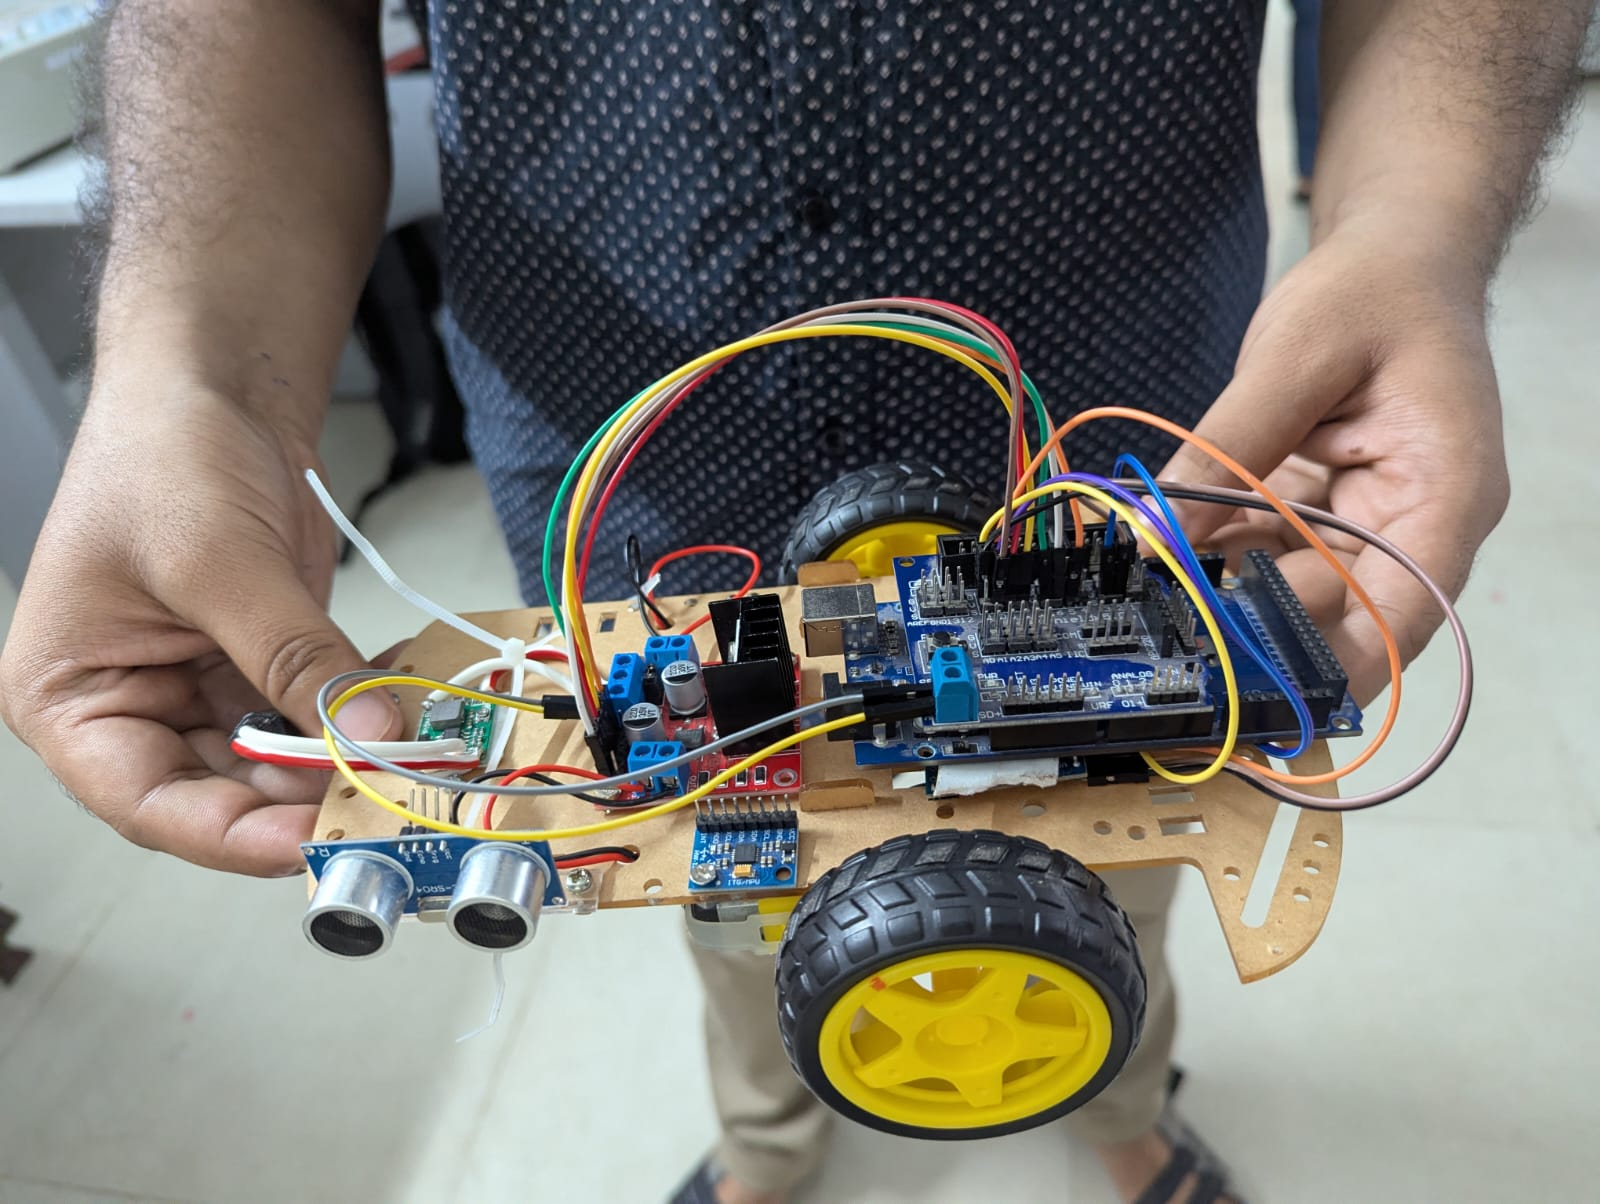
\includegraphics[width=\textwidth]{hardware_front.jpeg}
    \caption{Front perspective view of assembled platform}
    \label{fig_hw_front}
\end{subfigure}
\hfill
\begin{subfigure}[b]{0.48\textwidth}
    \centering
    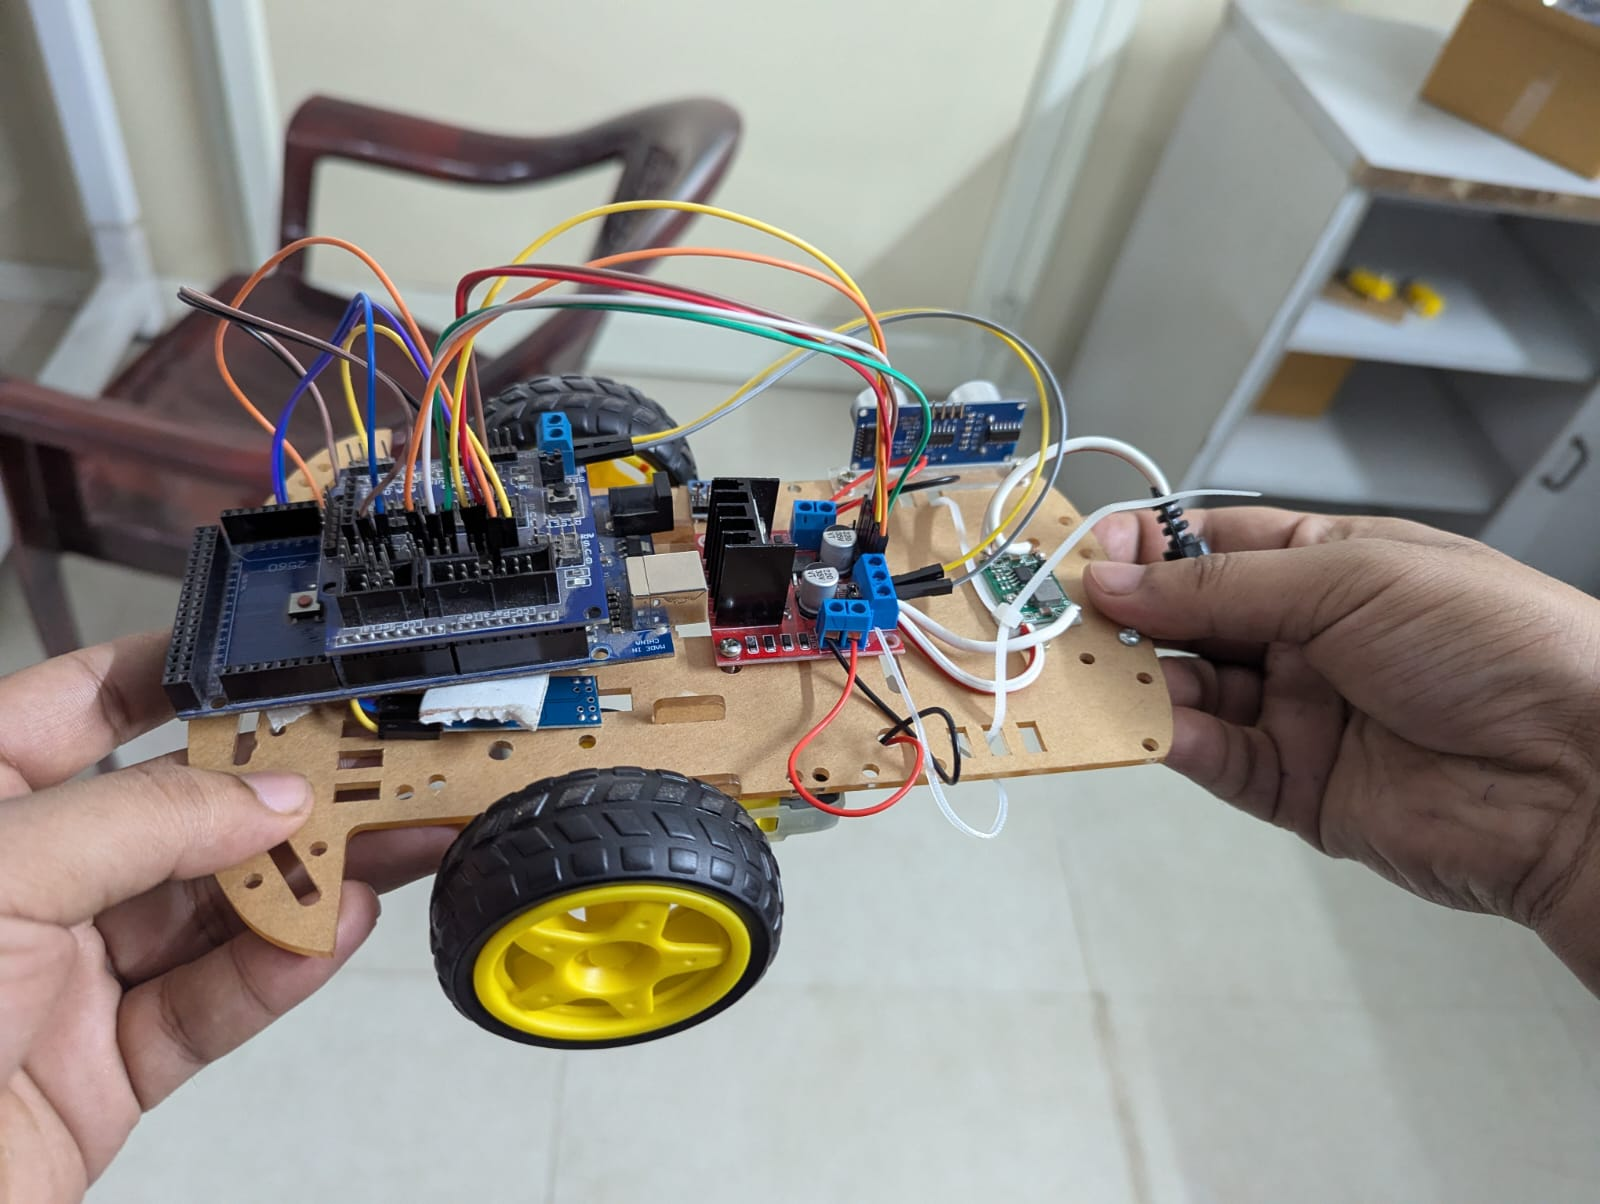
\includegraphics[width=\textwidth]{hardware_side.jpeg}
    \caption{Side oblique view showing wiring harness}
    \label{fig_hw_side}
\end{subfigure}

\vspace{0.3cm}
\begin{subfigure}[b]{0.48\textwidth}
    \centering
    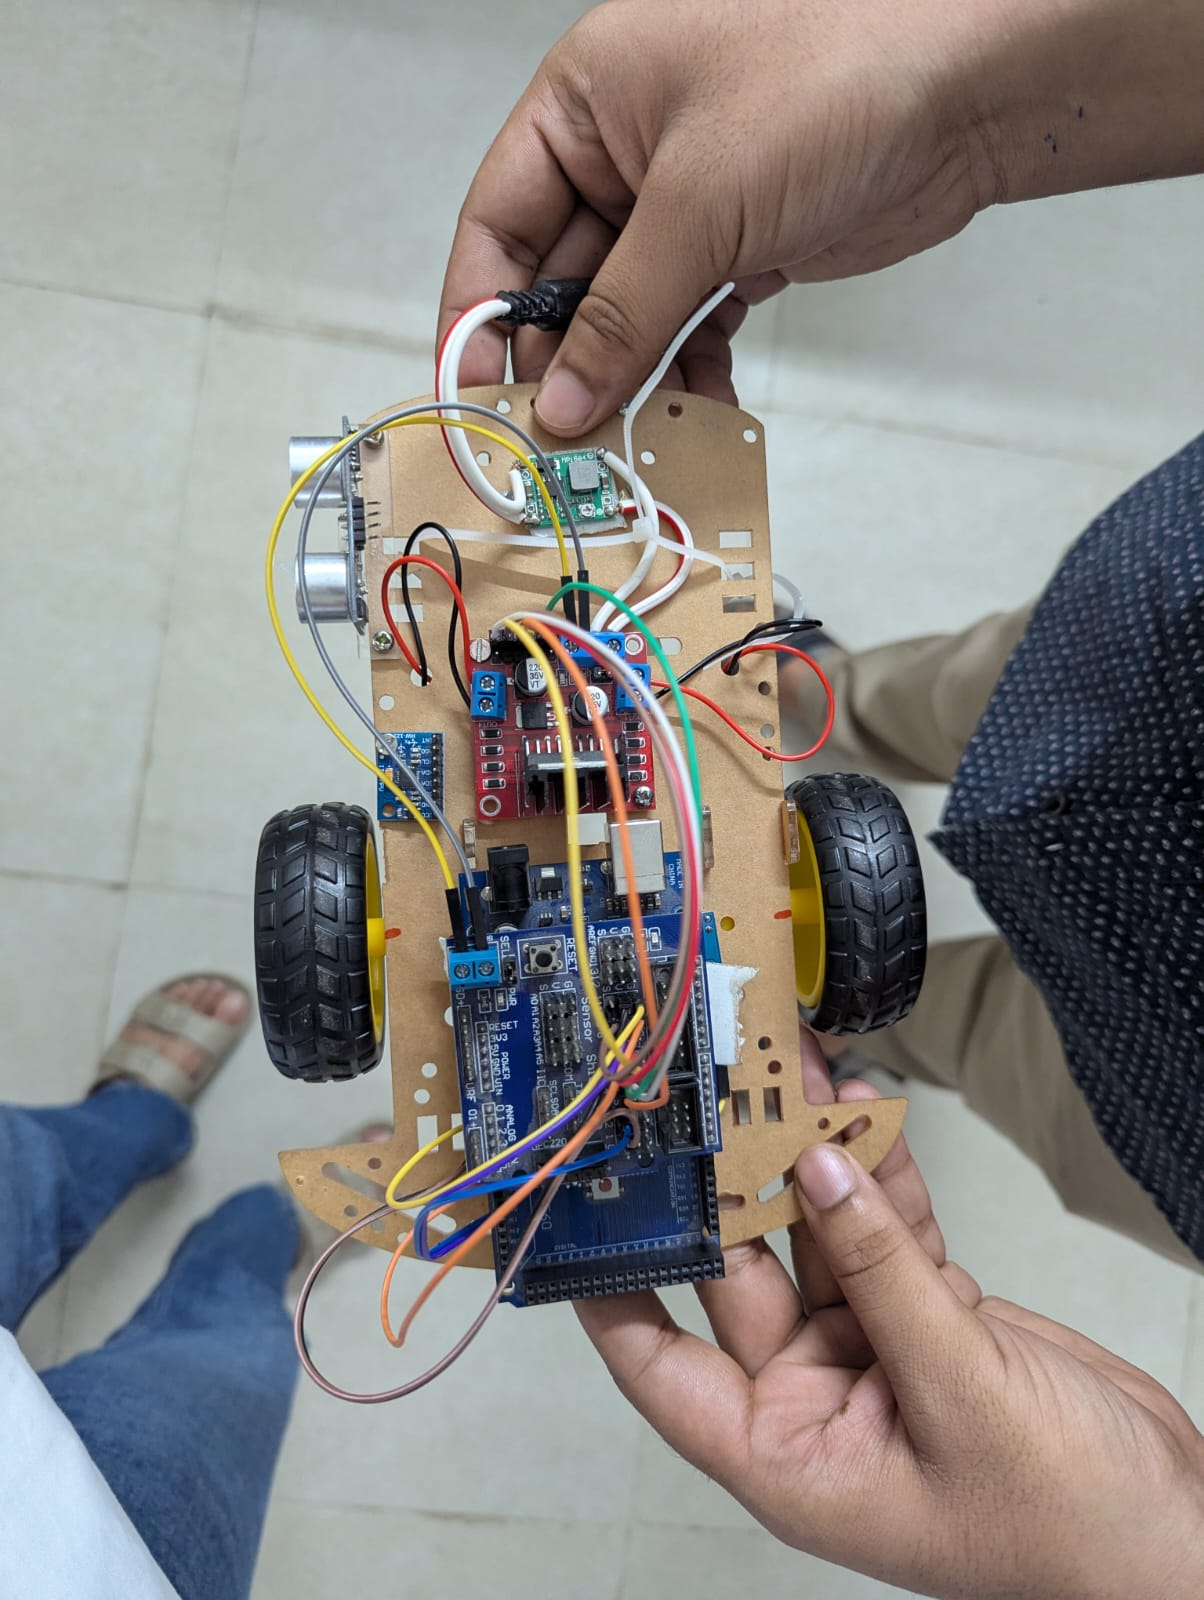
\includegraphics[width=\textwidth]{hardware_top.jpeg}
    \caption{Top layout showing driver and controller placement}
    \label{fig_hw_top}
\end{subfigure}
\caption{Photographs of the mobile robot platform illustrating the Arduino Mega 2560, sensor breakout shield, L298N motor driver, DC gear motors, and power regulation module.}
\label{fig_hardware}
\end{figure}

The physical assembly displays the dual-tier architecture of the mobile robot. As seen in Figure~\ref{fig_hw_front}, the front section carries an ultrasonic distance sensor alongside the wheel assemblies. Figure~\ref{fig_hw_side} shows the organized routing of colored jumper cables connecting the sensor shield headers to the L298N driver inputs and terminal blocks. Figure~\ref{fig_hw_top} shows the central placement of the L298N driver module equipped with its aluminum heatsink, positioned between the battery step-down regulator at the front and the Arduino Mega 2560 at the rear.

\subsection{Wiring Diagram}
Figure~\ref{fig_wiring} presents the complete circuit schematic linking the Arduino Mega 2560 microcontroller, the L298N dual H-bridge motor driver, the two direct current motors, and the reserved optical encoders.

\begin{figure}[H]
\centering
\resizebox{0.95\textwidth}{!}{%
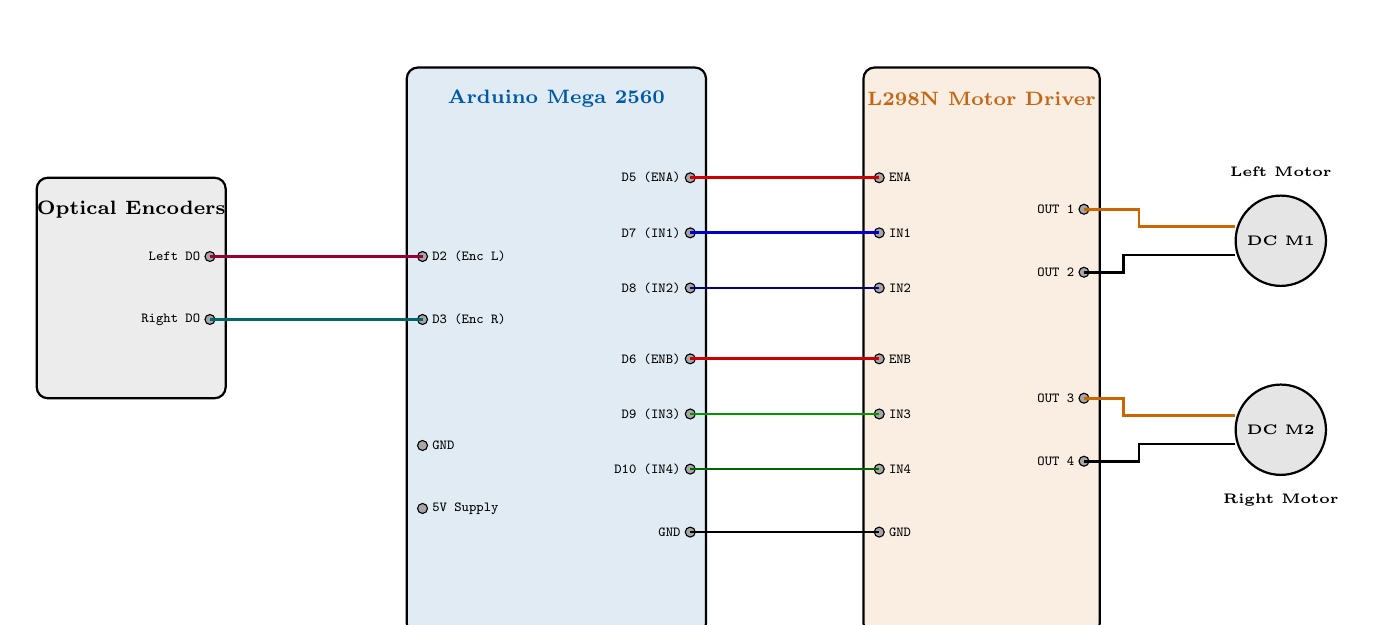
\begin{tikzpicture}[
    box/.style={draw=black, thick, rounded corners=4pt, fill=white, inner sep=5pt},
    pinlabel/.style={font=\ttfamily\tiny, text=black},
    wire/.style={line width=1.0pt}
]
    % Optical Encoders on Far Left
    \node[box, fill=gray!15, minimum width=2.4cm, minimum height=2.8cm] (enc) at (-5.4, 0.8) {};
    \node[font=\bfseries\scriptsize, text=black] at (-5.4, 1.8) {Optical Encoders};

    \node[pinlabel, anchor=east] (enc_l) at (-4.4, 1.2) {Left DO};
    \node[pinlabel, anchor=east] (enc_r) at (-4.4, 0.4) {Right DO};

    \foreach \p in {enc_l, enc_r} {
        \filldraw[fill=gray!70, draw=black] (\p.east) circle (1.8pt);
    }

    % Arduino Mega 2560
    \node[box, fill=arduinoblue!12, minimum width=3.8cm, minimum height=7.2cm] (mega) at (0, 0) {};
    \node[font=\bfseries\scriptsize, text=arduinoblue] at (0, 3.2) {Arduino Mega 2560};

    % Left pins on Mega (Encoders and Power)
    \node[pinlabel, anchor=west] (m_d2) at (-1.7, 1.2) {D2 (Enc L)};
    \node[pinlabel, anchor=west] (m_d3) at (-1.7, 0.4) {D3 (Enc R)};
    \node[pinlabel, anchor=west] (m_gnd_l) at (-1.7, -1.2) {GND};
    \node[pinlabel, anchor=west] (m_5v_l) at (-1.7, -2.0) {5V Supply};

    \foreach \p in {m_d2, m_d3, m_gnd_l, m_5v_l} {
        \filldraw[fill=gray!70, draw=black] (\p.west) circle (1.8pt);
    }

    % Right pins on Mega (Motor Driver Controls)
    \node[pinlabel, anchor=east] (m_p5) at (1.7, 2.2) {D5 (ENA)};
    \node[pinlabel, anchor=east] (m_p7) at (1.7, 1.5) {D7 (IN1)};
    \node[pinlabel, anchor=east] (m_p8) at (1.7, 0.8) {D8 (IN2)};
    \node[pinlabel, anchor=east] (m_p6) at (1.7, -0.1) {D6 (ENB)};
    \node[pinlabel, anchor=east] (m_p9) at (1.7, -0.8) {D9 (IN3)};
    \node[pinlabel, anchor=east] (m_p10) at (1.7, -1.5) {D10 (IN4)};
    \node[pinlabel, anchor=east] (m_gnd_r) at (1.7, -2.3) {GND};

    \foreach \p in {m_p5, m_p7, m_p8, m_p6, m_p9, m_p10, m_gnd_r} {
        \filldraw[fill=gray!70, draw=black] (\p.east) circle (1.8pt);
    }

    % L298N Driver
    \node[box, fill=driverorange!12, minimum width=3.0cm, minimum height=7.2cm] (l298) at (5.4, 0) {};
    \node[font=\bfseries\scriptsize, text=driverorange!90!black] at (5.4, 3.2) {L298N Motor Driver};

    % Left pins on L298N
    \node[pinlabel, anchor=west] (d_ena) at (4.1, 2.2) {ENA};
    \node[pinlabel, anchor=west] (d_in1) at (4.1, 1.5) {IN1};
    \node[pinlabel, anchor=west] (d_in2) at (4.1, 0.8) {IN2};
    \node[pinlabel, anchor=west] (d_enb) at (4.1, -0.1) {ENB};
    \node[pinlabel, anchor=west] (d_in3) at (4.1, -0.8) {IN3};
    \node[pinlabel, anchor=west] (d_in4) at (4.1, -1.5) {IN4};
    \node[pinlabel, anchor=west] (d_gnd)  at (4.1, -2.3) {GND};

    \foreach \p in {d_ena, d_in1, d_in2, d_enb, d_in3, d_in4, d_gnd} {
        \filldraw[fill=gray!70, draw=black] (\p.west) circle (1.8pt);
    }

    % Right pins on L298N (Motor outputs)
    \node[pinlabel, anchor=east] (d_out1) at (6.7, 1.8) {OUT 1};
    \node[pinlabel, anchor=east] (d_out2) at (6.7, 1.0) {OUT 2};
    \node[pinlabel, anchor=east] (d_out3) at (6.7, -0.6) {OUT 3};
    \node[pinlabel, anchor=east] (d_out4) at (6.7, -1.4) {OUT 4};

    \foreach \p in {d_out1, d_out2, d_out3, d_out4} {
        \filldraw[fill=gray!70, draw=black] (\p.east) circle (1.8pt);
    }

    % Motors
    \node[circle, draw=black, thick, fill=gray!20, minimum size=1.0cm, font=\tiny\bfseries] (m1) at (9.2, 1.4) {DC M1};
    \node[font=\tiny\bfseries, above=0.1cm of m1] {Left Motor};

    \node[circle, draw=black, thick, fill=gray!20, minimum size=1.0cm, font=\tiny\bfseries] (m2) at (9.2, -1.0) {DC M2};
    \node[font=\tiny\bfseries, below=0.1cm of m2] {Right Motor};

    % Wires: Encoders to Mega
    \draw[wire, color=purple!80!black] (enc_l.east) -- (m_d2.west);
    \draw[wire, color=teal!80!black] (enc_r.east) -- (m_d3.west);

    % Wires: Mega to L298N
    \draw[wire, color=red!80!black] (m_p5.east) -- (d_ena.west);
    \draw[wire, color=blue!80!black] (m_p7.east) -- (d_in1.west);
    \draw[wire, color=blue!50!black] (m_p8.east) -- (d_in2.west);
    \draw[wire, color=red!80!black] (m_p6.east) -- (d_enb.west);
    \draw[wire, color=green!60!black] (m_p9.east) -- (d_in3.west);
    \draw[wire, color=green!40!black] (m_p10.east) -- (d_in4.west);
    \draw[wire, color=black] (m_gnd_r.east) -- (d_gnd.west);

    % Wires: L298N to Motors
    \draw[wire, color=orange!80!black] (d_out1.east) -- ++(0.7,0) |- ($(m1.west)+(0,0.18)$);
    \draw[wire, color=black] (d_out2.east) -- ++(0.5,0) |- ($(m1.west)+(0,-0.18)$);
    \draw[wire, color=orange!80!black] (d_out3.east) -- ++(0.5,0) |- ($(m2.west)+(0,0.18)$);
    \draw[wire, color=black] (d_out4.east) -- ++(0.7,0) |- ($(m2.west)+(0,-0.18)$);

\end{tikzpicture}%
}
\caption{Circuit schematic and wiring diagram of the dual motor control system.}
\label{fig_wiring}
\end{figure}

The connections illustrated in Figure~\ref{fig_wiring} establish electrical signal transmission and power management. Microcontroller pulse width modulation pins 5 and 6 attach to enable terminals ENA and ENB on the L298N driver to regulate motor speed independently. Digital output pins 7 and 8 connect to input terminals IN1 and IN2 to set the rotational direction of the left direct current motor. Digital output pins 9 and 10 connect to terminals IN3 and IN4 to control the right direct current motor. Power driver output terminals OUT1 and OUT2 supply bidirectional current to the left motor, while terminals OUT3 and OUT4 power the right motor. Encoder signal outputs are wired to interrupt pins D2 and D3 for high-resolution pulse counting during future locomotion tasks. Common ground is shared across the Arduino board, the sensor shield, and the L298N driver to guarantee clean signal reference levels.

%--------------------------- Section 3 ---------------------------------
\section{Logic Used and System Flowchart}
The motor control logic coordinates velocity setpoints and directional switching using modular driver routines. Each motor is handled through a parameterized function that accepts the requested speed value and directional state. Speed commands are constrained within valid bounds before generating analog pulse width modulation signals, and direction parameters are mapped to corresponding logic states across the H-bridge input pins.

\subsection{System Flowchart}
Figure~\ref{fig_flowchart} illustrates the operational flow and execution states of the automated motor test routine.

\begin{figure}[H]
\centering
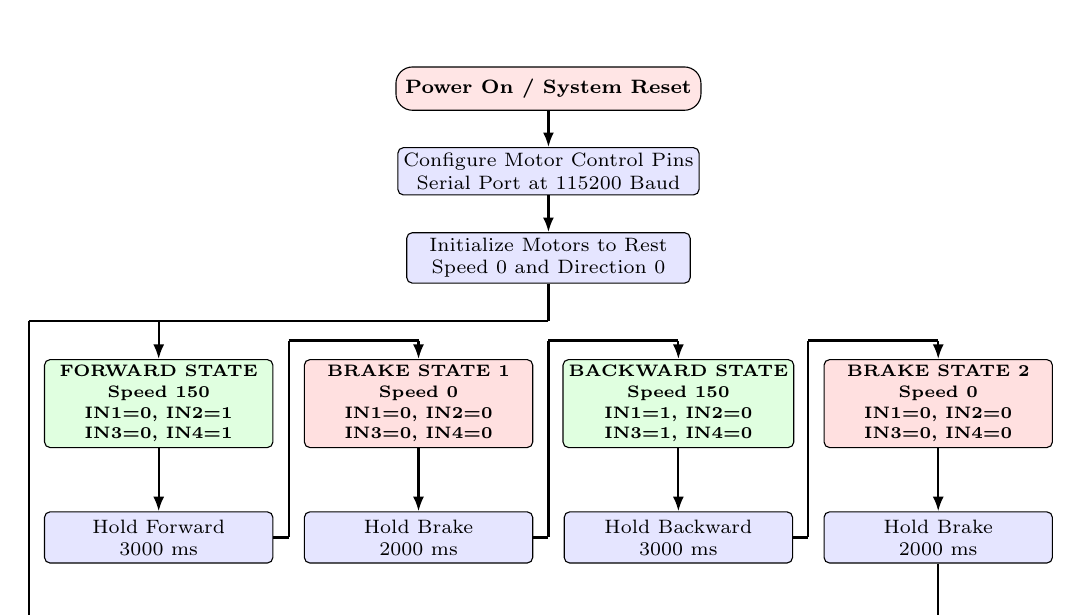
\begin{tikzpicture}[
    startstop/.style={rectangle, rounded corners=6pt, minimum width=3.4cm, minimum height=0.55cm, text centered, draw=black, fill=red!10, font=\scriptsize\bfseries},
    process/.style={rectangle, rounded corners=2pt, minimum width=3.6cm, minimum height=0.60cm, text centered, draw=black, fill=blue!10, font=\scriptsize, align=center, inner sep=2pt},
    actionbox/.style={rectangle, rounded corners=2pt, minimum width=2.9cm, minimum height=0.85cm, text centered, draw=black, fill=green!12, font=\fontsize{6.5}{7.5}\selectfont\bfseries, align=center, inner sep=2pt},
    stopbox/.style={rectangle, rounded corners=2pt, minimum width=2.9cm, minimum height=0.85cm, text centered, draw=black, fill=red!12, font=\fontsize{6.5}{7.5}\selectfont\bfseries, align=center, inner sep=2pt},
    arrow/.style={thick, -{Latex[scale=0.8]}},
    line/.style={thick}
]
    \node[startstop] (start) at (0, 6.2) {Power On / System Reset};
    \node[process] (init) at (0, 5.15) {Configure Motor Control Pins\\Serial Port at 115200 Baud};
    \node[process] (initial_stop) at (0, 4.05) {Initialize Motors to Rest\\Speed 0 and Direction 0};

    % 4 Execution States in the Cyclic Routine
    \node[actionbox] (b_fwd)   at (-4.95, 2.2) {FORWARD STATE\\Speed 150\\IN1=0, IN2=1\\IN3=0, IN4=1};
    \node[stopbox]   (b_stop1) at (-1.65, 2.2) {BRAKE STATE 1\\Speed 0\\IN1=0, IN2=0\\IN3=0, IN4=0};
    \node[actionbox] (b_bwd)   at ( 1.65, 2.2) {BACKWARD STATE\\Speed 150\\IN1=1, IN2=0\\IN3=1, IN4=0};
    \node[stopbox]   (b_stop2) at ( 4.95, 2.2) {BRAKE STATE 2\\Speed 0\\IN1=0, IN2=0\\IN3=0, IN4=0};

    % Delay blocks below action boxes
    \node[process, minimum width=2.9cm, minimum height=0.65cm] (d_fwd)   at (-4.95, 0.5) {Hold Forward\\3000 ms};
    \node[process, minimum width=2.9cm, minimum height=0.65cm] (d_stop1) at (-1.65, 0.5) {Hold Brake\\2000 ms};
    \node[process, minimum width=2.9cm, minimum height=0.65cm] (d_bwd)   at ( 1.65, 0.5) {Hold Backward\\3000 ms};
    \node[process, minimum width=2.9cm, minimum height=0.65cm] (d_stop2) at ( 4.95, 0.5) {Hold Brake\\2000 ms};

    % Connect top sequence
    \draw[arrow] (start) -- (init);
    \draw[arrow] (init) -- (initial_stop);

    % Connect initial stop to first state
    \draw[line] (initial_stop.south) -- (0, 3.25);
    \draw[line] (0, 3.25) -- (-4.95, 3.25);
    \draw[arrow] (-4.95, 3.25) -- (b_fwd.north);

    % Connect State to its Delay
    \draw[arrow] (b_fwd) -- (d_fwd);
    \draw[arrow] (b_stop1) -- (d_stop1);
    \draw[arrow] (b_bwd) -- (d_bwd);
    \draw[arrow] (b_stop2) -- (d_stop2);

    % Sequential progression between states
    \draw[line] (d_fwd.east) -- (-3.3, 0.5);
    \draw[line] (-3.3, 0.5) -- (-3.3, 3.0);
    \draw[line] (-3.3, 3.0) -- (-1.65, 3.0);
    \draw[arrow] (-1.65, 3.0) -- (b_stop1.north);

    \draw[line] (d_stop1.east) -- (0.0, 0.5);
    \draw[line] (0.0, 0.5) -- (0.0, 3.0);
    \draw[line] (0.0, 3.0) -- (1.65, 3.0);
    \draw[arrow] (1.65, 3.0) -- (b_bwd.north);

    \draw[line] (d_bwd.east) -- (3.3, 0.5);
    \draw[line] (3.3, 0.5) -- (3.3, 3.0);
    \draw[line] (3.3, 3.0) -- (4.95, 3.0);
    \draw[arrow] (4.95, 3.0) -- (b_stop2.north);

    % Loop back from final delay to first state
    \draw[line] (d_stop2.south) -- (4.95, -0.6);
    \draw[line] (4.95, -0.6) -- (-6.6, -0.6);
    \draw[line] (-6.6, -0.6) -- (-6.6, 3.25);
    \draw[line] (-6.6, 3.25) -- (-4.95, 3.25);

\end{tikzpicture}
\caption{Flow diagram of the dual H-bridge speed and direction control routine.}
\label{fig_flowchart}
\end{figure}

\subsection{Algorithmic Structure and Pseudocode}
Algorithm~\ref{algo_motor} outlines the firmware procedures executed by the microcontroller to manage both motor channels.

\begin{algorithm}[H]
\small
\SetAlFnt{\small}
\SetAlCapFnt{\small}
\SetAlCapNameFnt{\small}
\setlength{\algomargin}{1.2em}
\SetAlgoSkip{small}
\DontPrintSemicolon
\caption{Dual motor velocity and direction control algorithm}
\label{algo_motor}
Define pin designations for left motor enable and direction lines \\
Define pin designations for right motor enable and direction lines \\
Initialize nominal operating velocities leftSpeed and rightSpeed to 150 \\
\BlankLine
Procedure setMotor(speed, direction, inA, inB, enablePin) \\
\Indp
    Clamp speed value between lower bound 0 and upper bound 255 \\
    \uIf{direction == 1}{
        Write digital LOW to inA and digital HIGH to inB \tcp*{Forward}
    }
    \uElseIf{direction == -1}{
        Write digital HIGH to inA and digital LOW to inB \tcp*{Backward}
    }
    \Else{
        Write digital LOW to inA and digital LOW to inB \tcp*{Stop}
    }
    Apply pulse width modulation duty cycle speed to enablePin \\
\Indm
\BlankLine
Configure all motor pins as digital outputs and initialize serial link at 115200 baud \\
Halt both motors by setting speed to 0 and direction to 0 \\
\BlankLine
\While{true}{
    Execute setMotor for left motor with leftSpeed and forward direction \\
    Execute setMotor for right motor with rightSpeed and forward direction \\
    Hold forward motion for 3000 milliseconds \\
    Execute setMotor with speed 0 to brake both motors \\
    Hold stop for 2000 milliseconds \\
    Execute setMotor for left motor with leftSpeed and backward direction \\
    Execute setMotor for right motor with rightSpeed and backward direction \\
    Hold backward motion for 3000 milliseconds \\
    Execute setMotor with speed 0 to brake both motors \\
    Hold stop for 2000 milliseconds \\
}
\end{algorithm}

\subsection{H-Bridge Operating Principles}
The L298N module incorporates a dual full-bridge monolithic integrated circuit. Each internal bridge consists of four solid-state switching elements arranged in an H pattern with the motor windings connected across the central cross-arm. Controlling the state of diagonally opposed transistors determines current direction and rotation.

Table~\ref{tab_truth} presents the operational truth table governing motor control states for input pin combinations.

\begin{table}[H]
\centering
\begin{tabularx}{\textwidth}{@{}l l l l X@{}}
\toprule
\textbf{IN1 / IN3} & \textbf{IN2 / IN4} & \textbf{Enable} & \textbf{Driver State} & \textbf{Operational Motor Response} \\
\midrule
LOW & HIGH & PWM ($>0$) & Active Forward & Continuous forward rotation at set PWM velocity \\
HIGH & LOW & PWM ($>0$) & Active Reverse & Continuous reverse rotation at set PWM velocity \\
LOW & LOW & ANY & Dynamic Brake & Fast motor deceleration with windings tied to ground \\
HIGH & HIGH & ANY & Dynamic Brake & Fast motor deceleration with windings tied to supply \\
ANY & ANY & LOW (0) & Free Coast & Motor coast to rest with output stages disabled \\
\bottomrule
\end{tabularx}
\caption{H-Bridge switching logic and operational motor states.}
\label{tab_truth}
\end{table}

Speed control operates via pulse width modulation. The microcontroller timers toggle the enable line at a frequency of 490 hertz. The effective terminal voltage delivered to each motor winding equals the power rail voltage multiplied by the duty cycle ratio. A programmed value of 150 produces an effective duty cycle of 58.8 percent, delivering adequate initial current to overcome static friction and gear train resistance while maintaining smooth, controllable vehicular travel.

%--------------------------- Section 4 ---------------------------------
\section{Code}
The complete Arduino C++ firmware uploaded to the microcontroller is provided below.

\begin{lstlisting}
// ==========================================================
//        L298N DUAL MOTOR SPEED + DIRECTION CONTROL
//        Arduino Mega / Mega ADK
// ==========================================================
//
// LEFT MOTOR:
//   ENA -> D5
//   IN1 -> D7
//   IN2 -> D8
//
// RIGHT MOTOR:
//   ENB -> D6
//   IN3 -> D9
//   IN4 -> D10
//
// Encoder pins are reserved:
//   Left encoder  DO -> D2
//   Right encoder DO -> D3
//
// Speed range:
//   0   = STOP
//   255 = MAXIMUM
//
// Direction:
//   FORWARD
//   BACKWARD
//   STOP
// ==========================================================


// ---------------- PIN DEFINITIONS ----------------

// Left motor
const int ENA = 5;
const int IN1 = 7;
const int IN2 = 8;

// Right motor
const int ENB = 6;
const int IN3 = 9;
const int IN4 = 10;


// ---------------- MOTOR SETTINGS ----------------

// Speed: 0 to 255
int leftSpeed  = 150;
int rightSpeed = 150;


// ==========================================================
// MOTOR A (LEFT) CONTROL
// ==========================================================

void leftMotor(int speed, int direction)
{
  speed = constrain(speed, 0, 255);

  if (direction == 1)
  {
    // FORWARD
    digitalWrite(IN1, LOW);
    digitalWrite(IN2, HIGH);
  }
  else if (direction == -1)
  {
    // BACKWARD
    digitalWrite(IN1, HIGH);
    digitalWrite(IN2, LOW);
  }
  else
  {
    // STOP
    digitalWrite(IN1, LOW);
    digitalWrite(IN2, LOW);
  }

  analogWrite(ENA, speed);
}


// ==========================================================
// MOTOR B (RIGHT) CONTROL
// ==========================================================

void rightMotor(int speed, int direction)
{
  speed = constrain(speed, 0, 255);

  if (direction == 1)
  {
    // FORWARD
    digitalWrite(IN3, LOW);
    digitalWrite(IN4, HIGH);
  }
  else if (direction == -1)
  {
    // BACKWARD
    digitalWrite(IN3, HIGH);
    digitalWrite(IN4, LOW);
  }
  else
  {
    // STOP
    digitalWrite(IN3, LOW);
    digitalWrite(IN4, LOW);
  }

  analogWrite(ENB, speed);
}


// ==========================================================
// SETUP
// ==========================================================

void setup()
{
  pinMode(ENA, OUTPUT);
  pinMode(IN1, OUTPUT);
  pinMode(IN2, OUTPUT);

  pinMode(ENB, OUTPUT);
  pinMode(IN3, OUTPUT);
  pinMode(IN4, OUTPUT);

  Serial.begin(115200);

  // Start with motors stopped
  leftMotor(0, 0);
  rightMotor(0, 0);

  Serial.println("=================================");
  Serial.println("   MOTOR SPEED + DIRECTION TEST");
  Serial.println("=================================");
}


// ==========================================================
// LOOP
// ==========================================================

void loop()
{
  // --------------------------------------------------------
  // FORWARD
  // --------------------------------------------------------

  Serial.println("FORWARD");

  leftMotor(leftSpeed, 1);
  rightMotor(rightSpeed, 1);

  delay(3000);


  // --------------------------------------------------------
  // STOP
  // --------------------------------------------------------

  Serial.println("STOP");

  leftMotor(0, 0);
  rightMotor(0, 0);

  delay(2000);


  // --------------------------------------------------------
  // BACKWARD
  // --------------------------------------------------------

  Serial.println("BACKWARD");

  leftMotor(leftSpeed, -1);
  rightMotor(rightSpeed, -1);

  delay(3000);


  // --------------------------------------------------------
  // STOP
  // --------------------------------------------------------

  Serial.println("STOP");

  leftMotor(0, 0);
  rightMotor(0, 0);

  delay(2000);
}
\end{lstlisting}

\newpage
%--------------------------- Section 5 ---------------------------------
\section{Results}
The integrated mobile robot was tested under laboratory bench and floor conditions. The Arduino Mega 2560 continuously executed the speed and direction control firmware, generating real-time telemetry over the universal asynchronous receiver transmitter interface at 115200 baud.

Table~\ref{tab_results} summarizes the measured behavioral states observed during continuous testing of the four-phase cyclic routine.

\begin{table}[H]
\centering
\begin{tabularx}{\textwidth}{@{}lccccX@{}}
\toprule
\textbf{Phase} & \textbf{Left PWM} & \textbf{Right PWM} & \textbf{Left Dir} & \textbf{Right Dir} & \textbf{Observed Motion and Behavior} \\
\midrule
Phase 1 (3s) & 150 & 150 & Forward & Forward & Stable forward drive with straight vehicular trajectory \\
Phase 2 (2s) & 0 & 0 & Stop & Stop & Rapid deceleration and standstill under motor braking \\
Phase 3 (3s) & 150 & 150 & Backward & Backward & Uniform reverse motion matching forward velocity \\
Phase 4 (2s) & 0 & 0 & Stop & Stop & Complete vehicle arrest without inductive disturbance \\
\bottomrule
\end{tabularx}
\caption{Observed experimental motion states during the cyclic execution test.}
\label{tab_results}
\end{table}

Experimental testing verified that a pulse width modulation value of 150 successfully overcomes gearbox stiction and inertial load without inducing tire slippage. The two-second intermediate stopping period provides an essential dead-time interval that protects the H-bridge switching transistors from shoot-through current surges during polarity reversal. Serial monitor logs confirmed synchronized state switching in exact accordance with the programmed timing sequence.

%--------------------------- Section 6 ---------------------------------
\section{Video}
The recorded experimental demonstration verifying the operation of the dual H-bridge motor speed and direction control system is hosted on the institutional repository.

\vspace{0.4cm}
\begin{center}
\href{https://indianinstituteofscience.sharepoint.com/:v:/s/MN2072026-27Aug-Dec/IQBDHjg9-icaQKrUQQ8hURULAYgFpN8kbQRPvqOYy3tRWW0?e=3t7jld}{\large \textbf{Click Here to View the Motor Driver Demonstration Video}}
\end{center}

\vspace{0.4cm}
\noindent
The complete web link for manual browser access is provided below.

\vspace{0.2cm}
\noindent
{\footnotesize \url{https://indianinstituteofscience.sharepoint.com/:v:/s/MN2072026-27Aug-Dec/IQBDHjg9-icaQKrUQQ8hURULAYgFpN8kbQRPvqOYy3tRWW0?e=3t7jld}}

\end{document}
